\documentclass[twoside,a4paper]{article}
\usepackage{geometry}
\geometry{margin=1.5cm, vmargin={0pt,1cm}}
\setlength{\topmargin}{-1cm}
\setlength{\paperheight}{29.7cm}
\setlength{\textheight}{25.3cm}

% useful packages.
\usepackage{amsfonts}
\usepackage{amsmath}
\usepackage{amssymb}
\usepackage{amsthm}
\usepackage{enumerate}
\usepackage{graphicx}[H]
\usepackage{multicol}
\usepackage{fancyhdr}
\usepackage{layout}
\usepackage{float}

% some common command
\newcommand{\dif}{\mathrm{d}}
\newcommand{\avg}[1]{\left\langle #1 \right\rangle}
\newcommand{\difFrac}[2]{\frac{\dif #1}{\dif #2}}
\newcommand{\pdfFrac}[2]{\frac{\partial #1}{\partial #2}}
\newcommand{\OFL}{\mathrm{OFL}}
\newcommand{\UFL}{\mathrm{UFL}}
\newcommand{\fl}{\mathrm{fl}}
\newcommand{\op}{\odot}
\newcommand{\Eabs}{E_{\mathrm{abs}}}
\newcommand{\Erel}{E_{\mathrm{rel}}}

\begin{document}

\pagestyle{fancy}
\fancyhead{}
\lhead{Jovi Wong(3180104829)}
\chead{Math Software \#day3}
\rhead{2020/7/8}


\section*{I. Relation between Image and Matrix}
\subsection*{I-a. swith RGB channel with each other}
\begin{figure}[H]
\centering
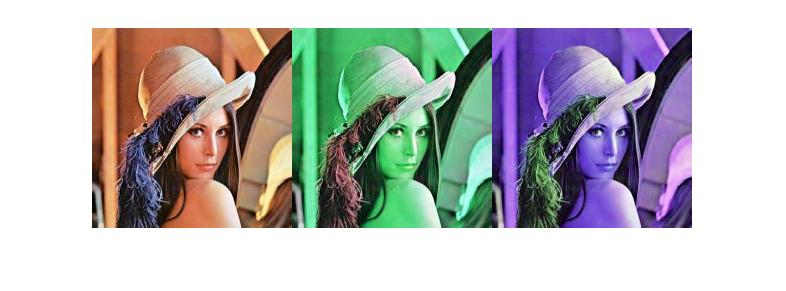
\includegraphics[width=7in]{channel.jpg}
\end{figure}
\subsection*{I-b. add operation}
\begin{figure}[H]
\centering
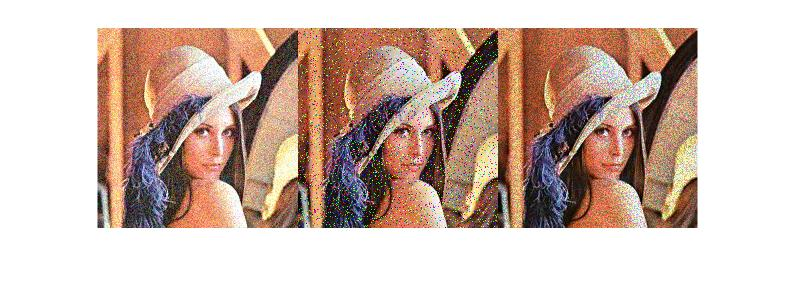
\includegraphics[width=7in]{addnoise.jpg}
\end{figure}
Add different kinds of noise(Gaussian, salt\&pepper and speckle from left to right) to the original picture.
\subsection*{I-c. multiply operation}
\begin{figure}[H]
\centering
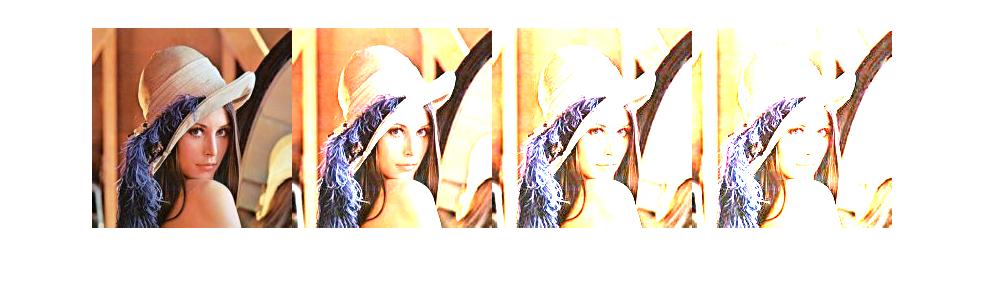
\includegraphics[width=7in]{multiply.jpg}
\end{figure}
Value is amplified as $\times$ 1, $\times$ 2, $\times$ 3, $\times$ 4 times from left to right. 
\subsection*{I-d. rotate operation}
\begin{figure}[H]
\centering
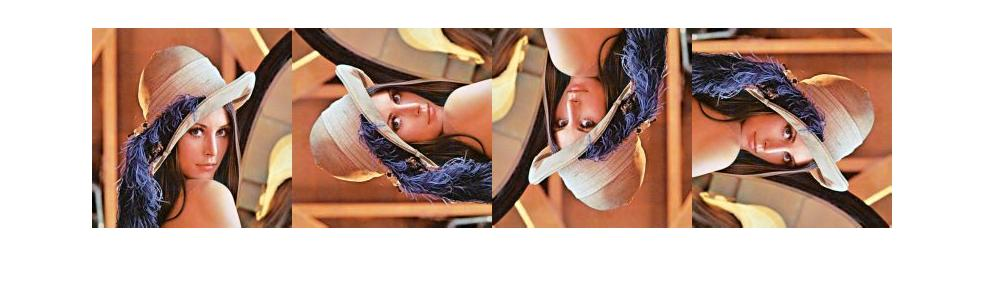
\includegraphics[width=7in]{rotate.jpg}
\end{figure}
Rotate the matrix along with the figure.
\section*{II. Global and Local Traits}
\subsection*{II-a. histogram}
\begin{figure}[H]
\centering
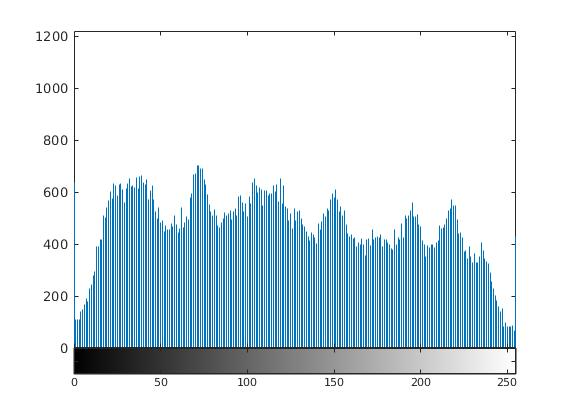
\includegraphics[width=6in]{hist.jpg}
\end{figure}
\subsection*{II-b. Fourier transform}
\begin{figure}[H]
\centering
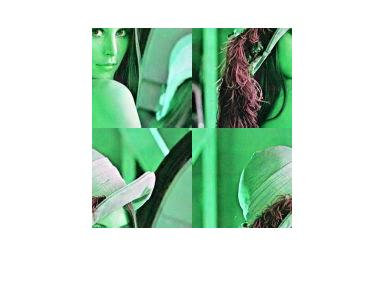
\includegraphics[width=5in]{fft.jpg}
\caption{fftshift}
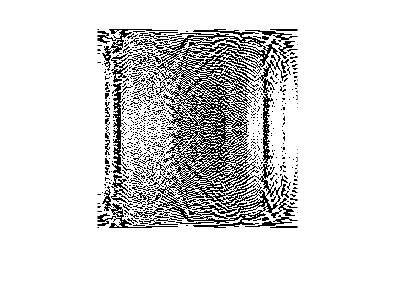
\includegraphics[width=5in]{realfft.jpg}
\caption{fft}
\end{figure}
This result is got by transforming the red channel.
\subsection*{II-c. filter}
\begin{figure}[H]
\centering
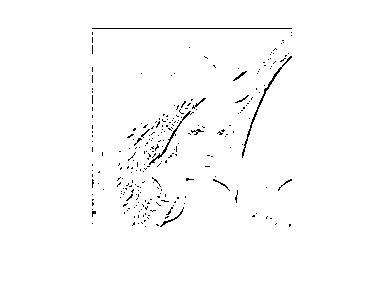
\includegraphics[width=6in]{filter.jpg}
\end{figure}
Process the picture in terms of the green channel.
\section*{III. Basic Operation}
\subsection*{III-a. divide}
\begin{figure}[H]
\centering
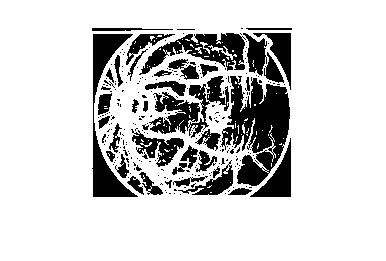
\includegraphics[width=6in]{divide.jpg}
\caption{threshold=5}
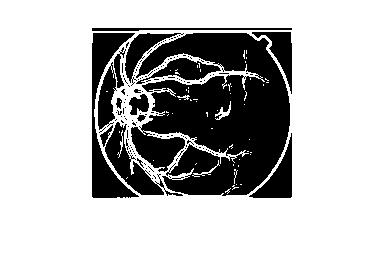
\includegraphics[width=6in]{divide10.jpg}
\caption{threshold=10}
\end{figure}

\subsection*{III-b fix}
\begin{figure}[H]
\centering
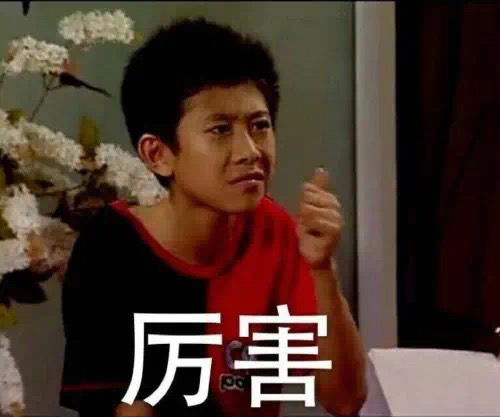
\includegraphics[width=4in]{before.jpg}
\caption{before}
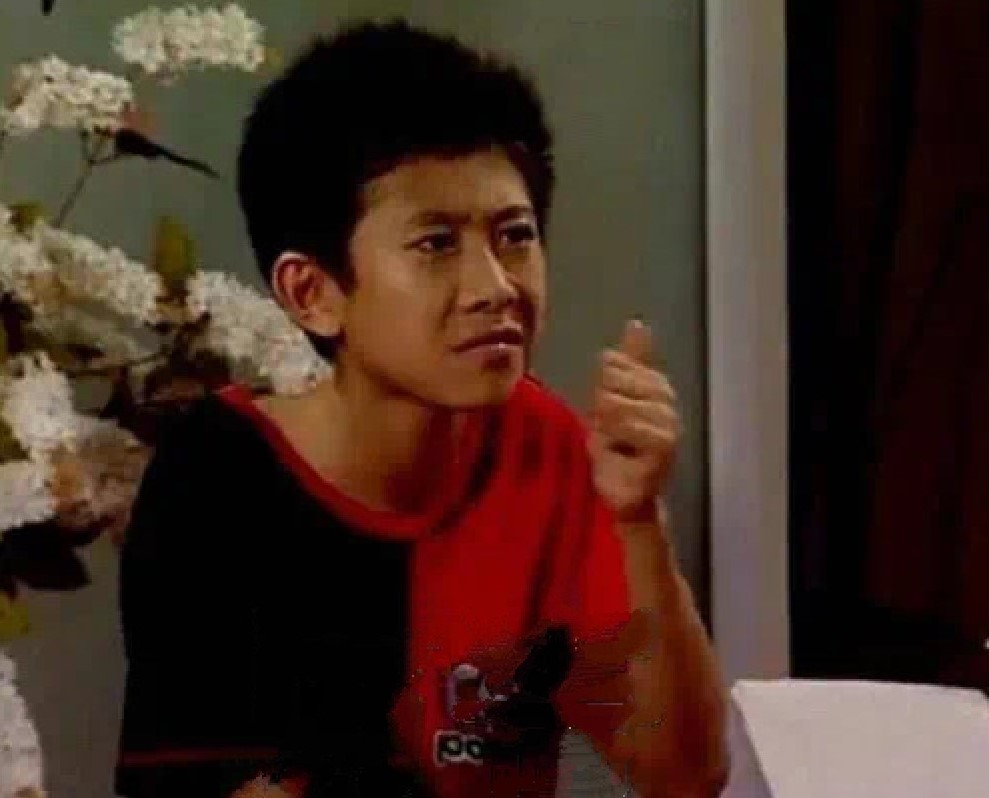
\includegraphics[width=4in]{after.jpg}
\caption{after}
\end{figure}
\end{document}

%%% Local Variables: 
%%% mode: latex
%%% TeX-master: t
%%% End: 
